\documentclass{article}
\usepackage{ctex}
\usepackage{geometry}
\geometry{top = 2cm, left = 1cm, right = 1cm, bottom = 2cm}
\usepackage{amsmath,amssymb,amsthm,amsfonts}
\usepackage{abstract}
\usepackage{siunitx}
\usepackage{graphicx}
\usepackage{booktabs}
\usepackage{appendix}
\usepackage{hyperref}

\renewcommand{\appendixpagename}{附录}


\title{高纯锗(HPGe)$\gamma$射线谱仪}
\author{钱思天 2001112187}
\begin{document}
    \maketitle
    \begin{abstract}
        本实验利用了高纯锗(HPGe)谱仪探测器,对$^{60}\text{Co},^{152}\text{Eu}$源、环境本底以及矿渣样本进行测量。
        通过对$^{152}\text{Eu}$源的测量,对探测系统进行了相对效率刻度,而后,通过对$^{60}\text{Co}$源的测量,对实验测量系统做了绝对效率刻度。而后,通过调节放大倍数并重新刻度,让探测器能够探测矿渣中的$\gamma$射线,进而判断出矿渣中所含有的元素。
        \newline
        \newline
        {\emph{ 关键词:\ 高纯锗$\gamma$射线谱仪、探测效率刻度、未知成分探测 }\rm}

    \end{abstract}

    \section{背景简介}
    \subsection{高纯锗$\gamma$射线谱仪}
    $\gamma$射线是原子核衰变或裂变时放出的辐射,本质上它是一种能量比可见光和$X$射线高得
多的电磁辐射。利用$\gamma$射线与物质相互作用的规律,人们已设计出多种类型的$\gamma$射线的探测
器。用于测量$\gamma$射线能量和强度的仪器称为$\gamma$能谱仪,谱仪一般有射线探测器和电子学系统
两大部分。最常用的有 NaI(Tl)闪烁谱仪和高纯锗(HPGe)半导体谱仪。闪烁探测器是利用某些
物质在射线作用下发光的特性来探测射线的仪器。HPGe 探测器是利用$\gamma$光子与探测介质原
子发生相互作用产生次级电子,通过次级电子在介质中的电离效应来探测射线的仪器。本实
验介绍一种高分辨率的高纯锗$\gamma$谱仪。
高纯锗探测器(High-Purity Germanium 简称 HPGe 探测器)实质上是利用纯度极高的锗制
成的 P-N 探测器。由于锗的纯度极高,也就是杂质浓度很低,因而电阻率很大,可得到较厚
的耗尽层,又由于锗的原子序数高,适合于探测$\gamma$射线。HPGe 探测器具有能量分辨率极高
的优点,所以它被广泛应用于$\gamma$射线能谱的测量,使$\gamma$谱学的面貌发生了根本的变化。
近年来,在核谱学、核反应、核工程和核技术应用等方面,HPGe 探测器已成为分析复
杂$\gamma$能谱的不可缺少的工具。
\subsection{实验目的}
\begin{enumerate}
    \item 了解高纯锗(HPGe)γ射线谱仪的原理、一般操作以及数据采集、处理的方法等;
    \item 利用$^{60}\text{Co}$,$^{152}\text{Eu}$做探测效率刻度;
    \item 测定未知样品的种类、活度。
\end{enumerate}
\section{实验介绍}
\subsection{实验装置}
本实验用到的实验装置比较简单,有:
\begin{enumerate}
    \item 高纯锗谱仪一套;
    \item NIM机箱、插件式高压电源、低压电源、主放大器各一个;
    \item 多道数据采集以及微机系统一套。
    \item $^{60}\text{Co},^{152}\text{Eu}$放射源各一个;
    \item 未知矿渣样品及固定装置一套。
\end{enumerate}
\subsection{实验操作}
鉴于上一位同学实验结束时的状况,实验步骤调整如下:
\begin{enumerate}
    \item 连接电子学线路,
检查无误后给高纯锗探头加高压至$3500\si{V}$。并且沿用上一位同学成功的放大倍数$(50\times1.12)$。
    \item 测定环境本底与矿渣样品能谱,各20分钟。
    \item 测量$^{152}\text{Eu}$十分钟,利用此数据及接下来测量的$^{60}\text{Co}$数据进行刻度。
    \item 将主放大器的放大倍数调至两倍$(100\times 1.12)$,而后分别测量$^{60}\text{Co},^{152}\text{Eu}$及环境本底各10分钟,并利用他们进行刻度。
\end{enumerate}
\section{数据处理}
\subsection{利用$^{60}\text{Co}$的测量结果,计算谱仪的相关性能参数}
$^{60}\text{Co}$的测量谱如图\ref{fig:60Co},根据测量结果,可以计算出谱仪的相关性能参数,如谱仪分辨率,峰康比和相对探测效率。
\begin{figure}[htbp]
    \centering
    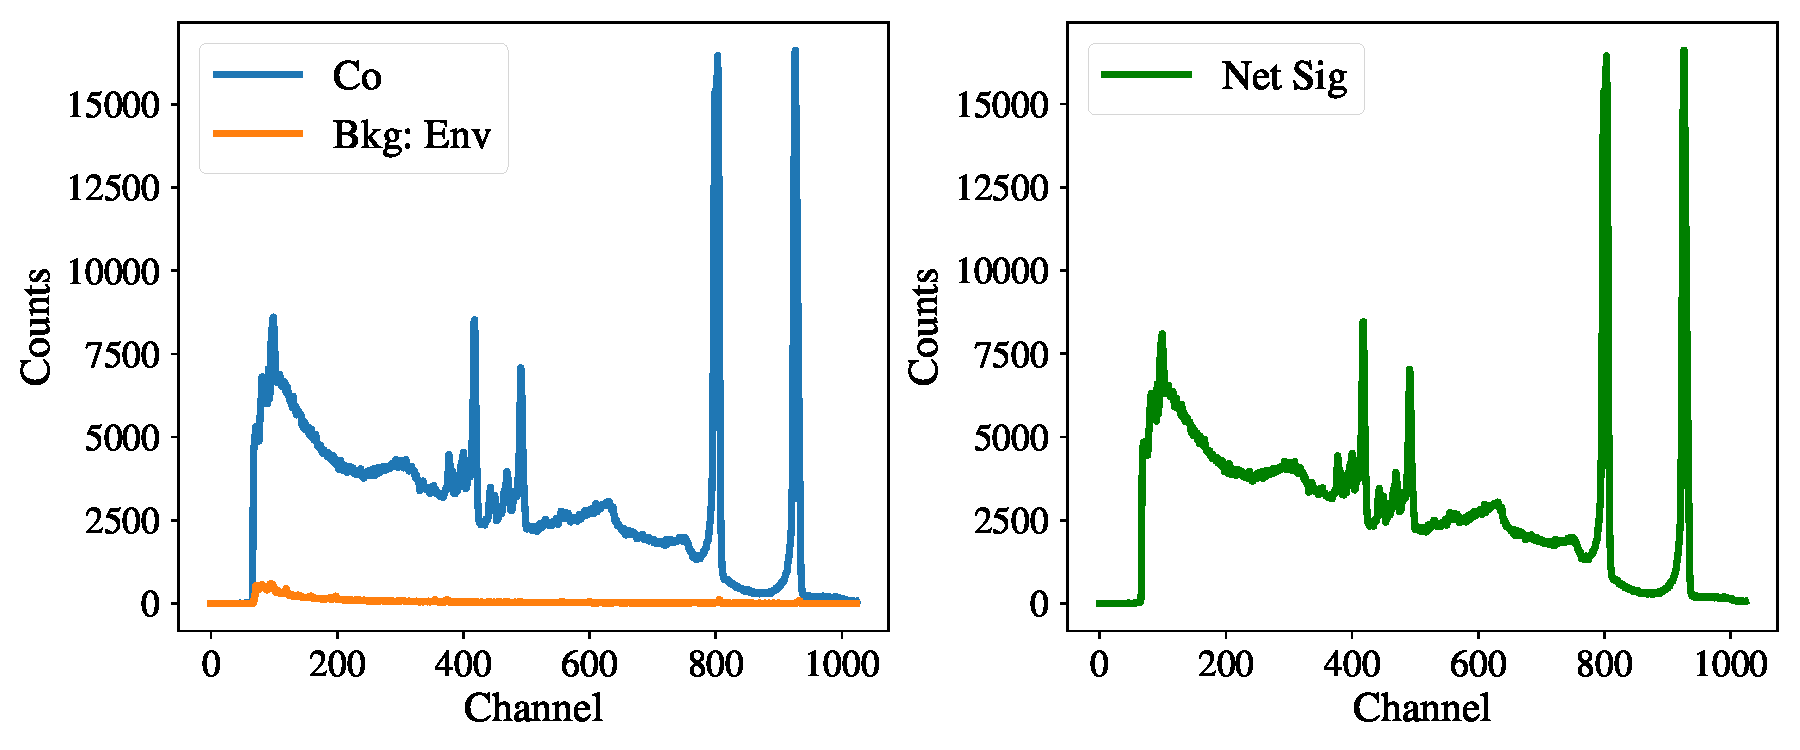
\includegraphics[width=\textwidth]{../plots/Co_net.pdf}
    \caption{$^{60}\text{Co}$放射源的测量结果\label{fig:60Co}}
\end{figure}
为了测算谱仪分辨率等,需要采用$^{60}\text{Co}$的两个特征峰,如图\ref{fig:60Co2Peak}。
\begin{figure}
    \centering
    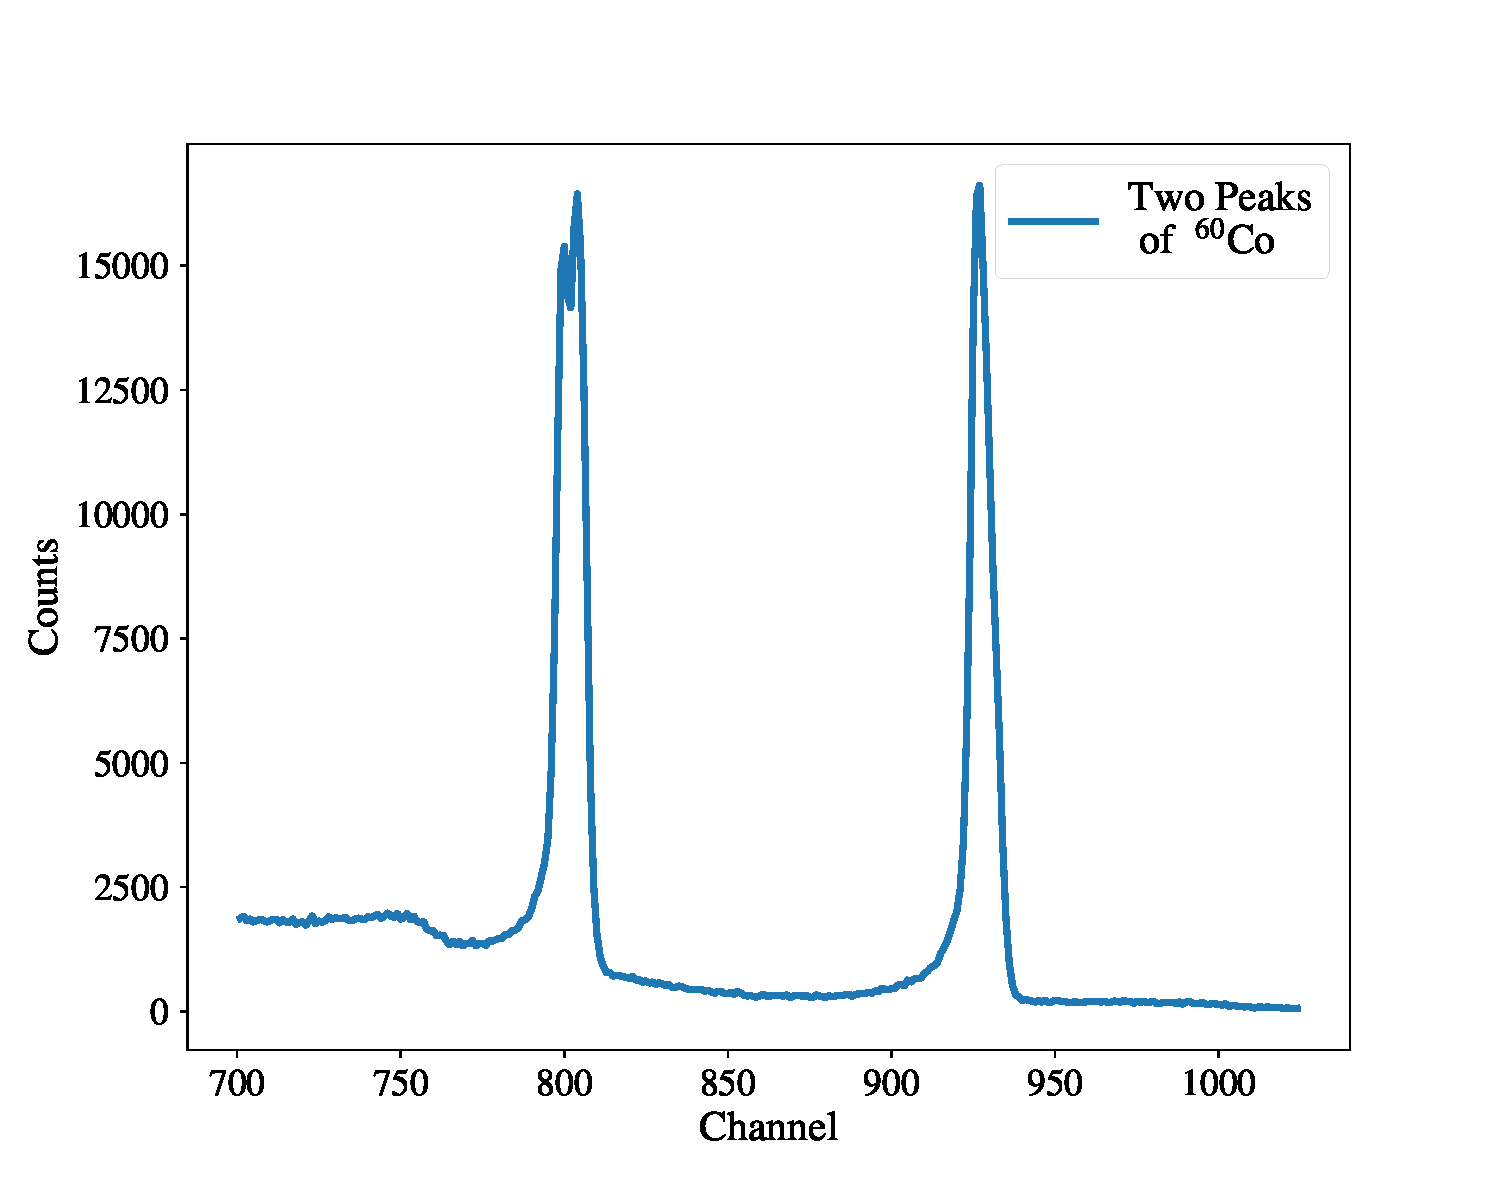
\includegraphics[width=0.6\textwidth]{../plots/Co_two_Peak.pdf}
    \caption{$^{60}\text{Co}$的两个特征峰\label{fig:60Co2Peak}}
\end{figure}
利用PHA18软件进行寻峰操作,可得结果如表\ref{tab:60Co},易知峰No.2为$1.33\si{MeV}$全能峰。其他的测量结果为
\begin{enumerate}
    \item 康普顿平台平均计数:4459.5;
    \item 活时$\si{528 s}$。
\end{enumerate}
\begin{table}[htbp]
    \centering
    \caption{$^{60}\text{Co}$的两个峰的测量结果\label{tab:60Co}}
    \begin{tabular}{rrrrrr}
\toprule
Peak &  Channel &  FWHM &  Peak Counts &  Peak Area & $E[\si{KeV}]$\\
\midrule
No.1    &      803 &   9.9 &        16472 &     193183 & 1173.2 \\
No.2    &      926 &   7.7 &        16633 &     149863 & 1332.5\\
\bottomrule
\end{tabular}
\end{table}
计算可得:
\begin{enumerate}
    \item 谱仪的能量分辨
    \begin{equation}
        \text{FWHM}*\frac{1332.5-1173.2}{826-803} = 9.97\si{KeV}
    \end{equation}
\item 峰康比:3.73;
\item 相对探测效率:
\begin{equation}
    \varepsilon_{ref} = \frac{S}{Dt} = 0.3\%
\end{equation}
\end{enumerate}
\subsection{刻度}
原则上说,既然道址和能量存在线性正比关系,那么最少利用两个点就可以进行刻度。仅利用$^{60}\text{Co}$刻度的结果为:
\begin{equation}
    E = 1.2591*\text{Ch} + 133.22
\end{equation}
但是,仅仅利用$^{60}\text{Co}$能谱的两个峰进行刻度,结果难免会有测量误差导致的偏差。

对$^{152}\text{Eu}$的测量结果如图\ref{fig:152Eu_Full}所示。
\begin{figure}[htbp]
    \centering
    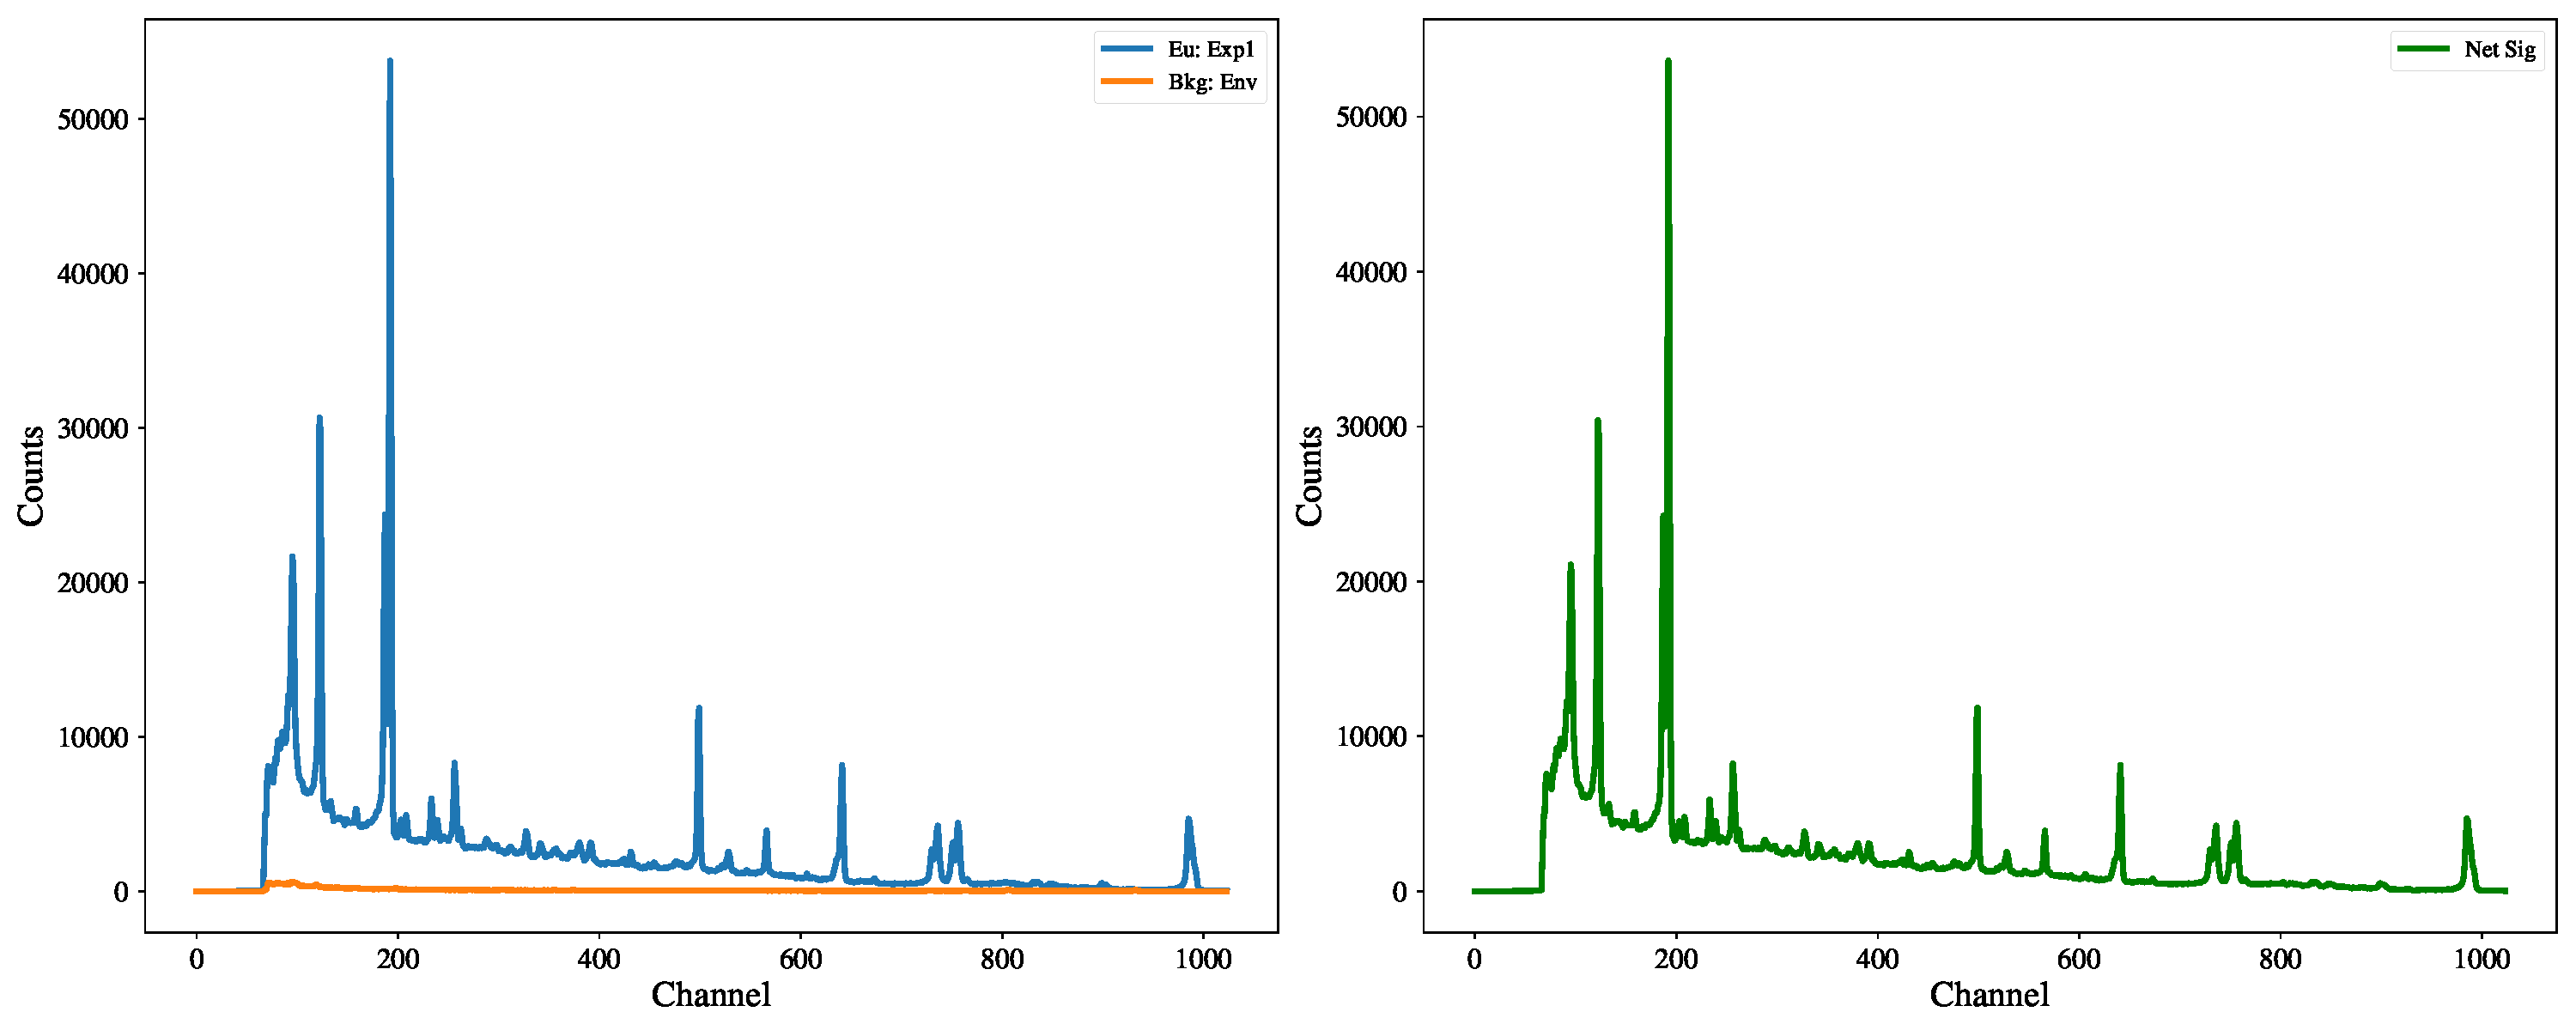
\includegraphics[width=\textwidth]{../plots/Eu_full_net.pdf}
    \caption{$^{152}\text{Eu}$第一次刻度的测量结果\label{fig:152Eu_Full}}
\end{figure}

如果利用上述$^{60}\text{Co}$进行刻度的结果对$^{152}\text{Eu}$进行粗测,结果如图\ref{fig:Roughly_Cali_full}。
\begin{figure}
    \centering
    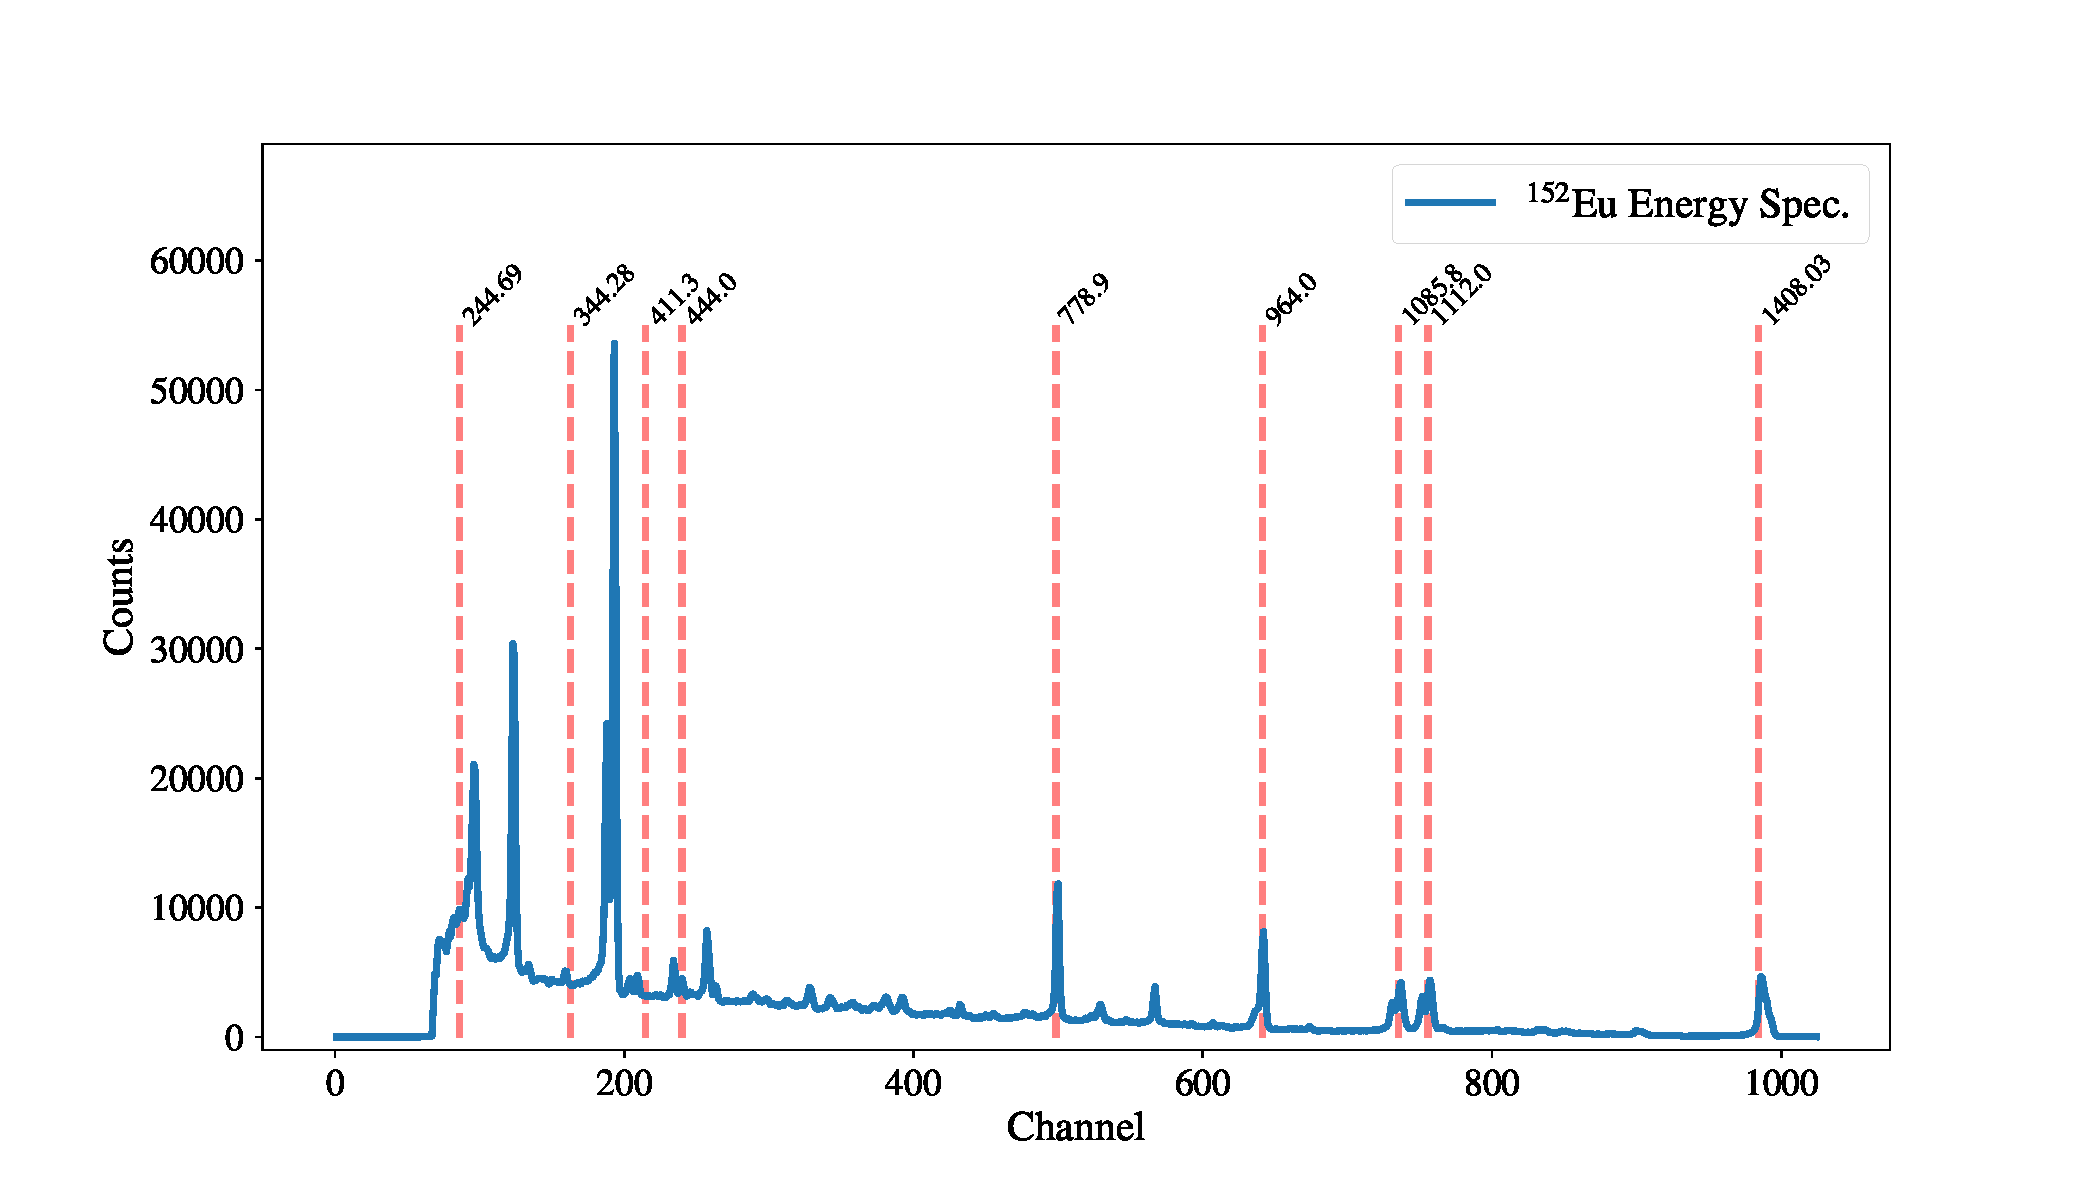
\includegraphics[width=\textwidth]{../plots/Roughly_Cali_full.pdf}
    \caption{利用$^{60}\text{Co}$的粗刻度结果对$^{152}\text{Eu}$的峰位进行预测,并和测量结果进行比较\label{fig:Roughly_Cali_full}}
\end{figure}

在高能区,粗测的刻度结果能够很好的解释实验观察到的峰位。但是能量较低的区间,则难以令人满意,这可能是由于低能区的响应不够线性带来的。因此,我们选用高能区的五个峰位,加上$^{60}\text{Co}$的两个峰进行刻度。$^{152}\text{Eu}$在这一阶段的测量数据记录如表\ref{tab:152Eu_full}。
\begin{table}[htbp]
    \centering
    \caption{$^{152}\text{Eu}$的测量结果\label{tab:152Eu_full}}
    \begin{tabular}{rrrrrrrr}
\toprule
Peak &  Channel &  Peak Area: $S$ &  Probability: $K$ &        $E[\si{KeV}]$ &          $S/K$ &  $\ln(S/K)$ &  $\ln(E)$ \\
\midrule
1    &      985 &      31800 &      0.20850 &  1408.03 &   152517.986 &   11.935 &  7.250 \\
2    &      756 &      23924 &      0.13560 &  1112.00 &   176430.678 &   12.081 &  7.014 \\
3    &      736 &      22745 &      0.10160 &  1085.80 &   223868.110 &   12.319 &  6.990 \\
4    &      641 &      31479 &      0.14620 &   964.00 &   215314.637 &   12.280 &  6.871 \\
5    &      499 &      30256 &      0.12960 &   778.90 &   233456.790 &   12.361 &  6.658 \\
6    &      256 &      20451 &      0.03121 &   444.00 &   655270.747 &   13.393 &  6.096 \\
7    &      233 &       9357 &      0.02230 &   411.30 &   419596.413 &   12.947 &  6.019 \\
8    &      192 &     197370 &      0.26580 &   344.28 &   742550.790 &   13.518 &  5.841 \\
9    &      122 &      83933 &      0.07510 &   244.69 &  1117616.511 &   13.927 &  5.500 \\
10   &       95 &     115823 &      0.28370 &   121.78 &   408258.724 &   12.920 &  4.802 \\
\bottomrule
\end{tabular}
\end{table}

根据实验数据,可得刻度为:
\begin{equation}
    E = 1.2945*\text{Ch} + 133.41
\end{equation}
刻度结果如图\ref{fig:Full_Fit}。
\begin{figure}[htbp]
    \centering
    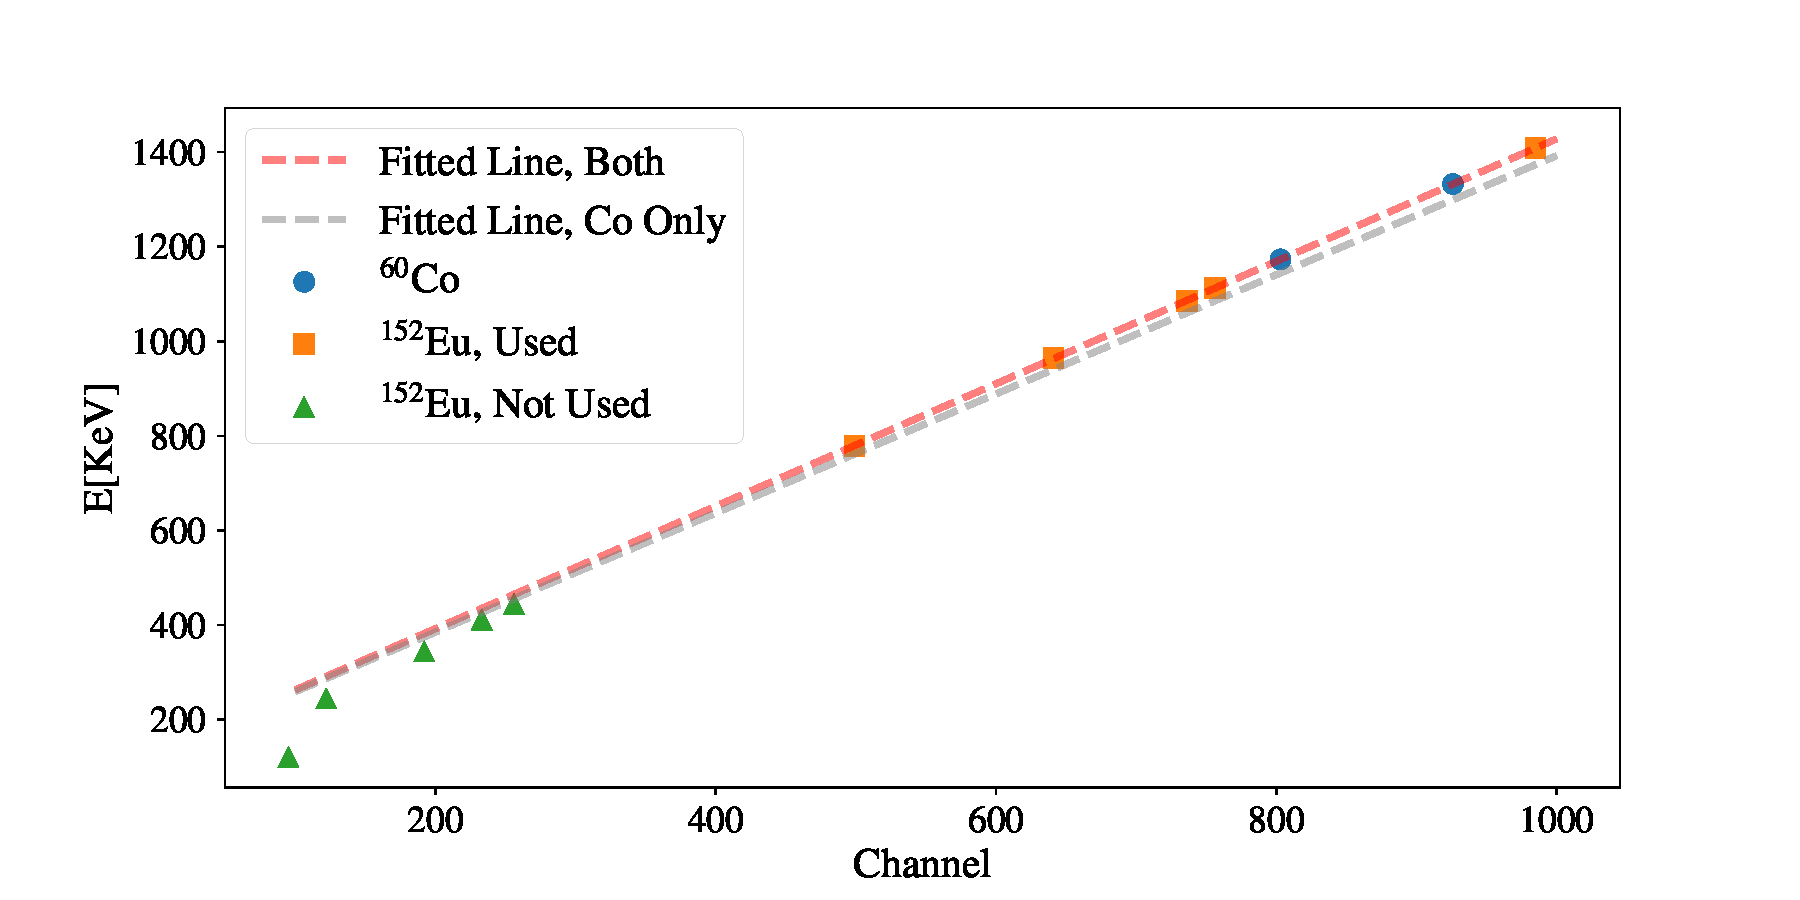
\includegraphics[width=\textwidth]{../plots/Full_Fit.pdf}
    \caption{本部分的刻度结果\label{fig:Full_Fit}}
\end{figure}
同时,也可得相对效率曲线如图\ref{fig:Relative}。考虑到低能区的响应不是很好,我们去除了低能的离群点。得到相对效率曲线如下:
\begin{equation}
    \ln(S/K) = -1.1274\ln(E) + 20.0469
\end{equation}
\begin{figure}[htbp]
    \centering
    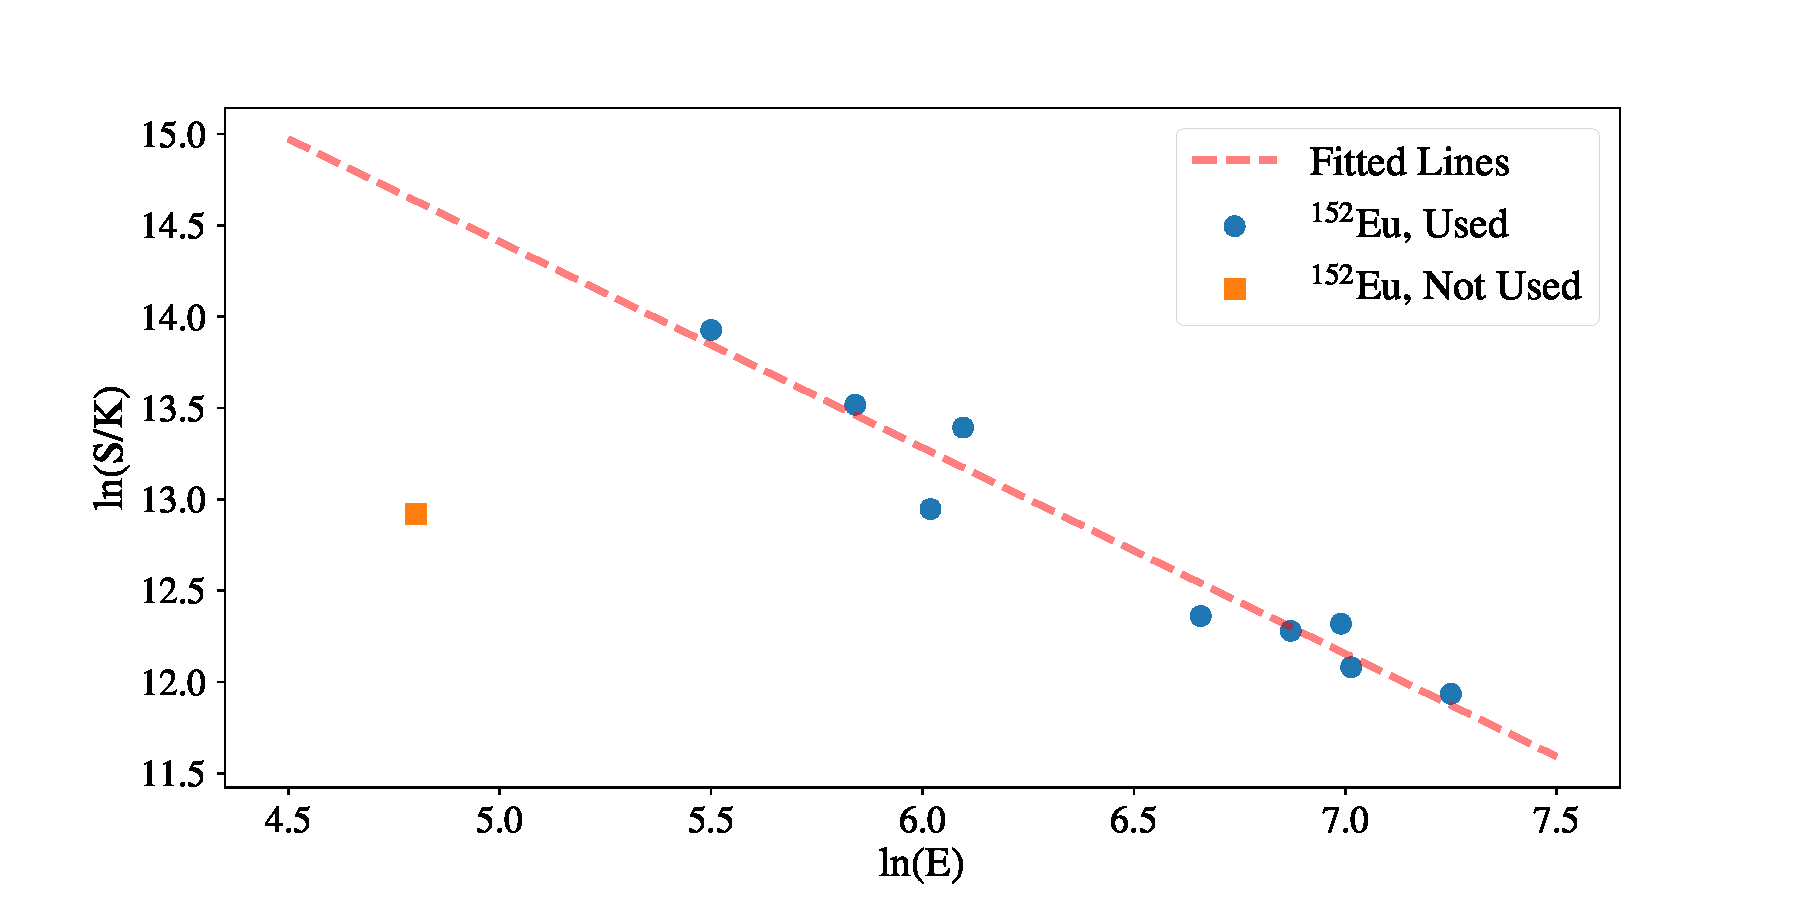
\includegraphics[width=\textwidth]{../plots/Relative.pdf}
    \caption{相对效率曲线$\ln(S/K)-\ln(E)$\label{fig:Relative}}
\end{figure}
\subsection{绝对效率曲线}
    对谱线的绝对效率值可以进行如下计算:
    \begin{equation}
        \begin{aligned}
            \varepsilon_i = \varepsilon_0\times(\frac{S_i}{K_i}/\frac{S_0}{K_0})
        \end{aligned}
    \end{equation}
    将$^{60}\text{Co}$的全能峰的峰位代入,可以得到
    \begin{equation}
        \frac{S_0}{K_0} \approx 152583.73
    \end{equation}
    由此,可以得到绝对探测效率公式为
    \begin{equation}
        \varepsilon_i = 1.97\times 10^{-8}(\frac{S_i}{K_i})
    \end{equation}
    而后,可以做出绝对效率曲线如图\ref{fig:Absolute}。
    \begin{figure}
        \centering
        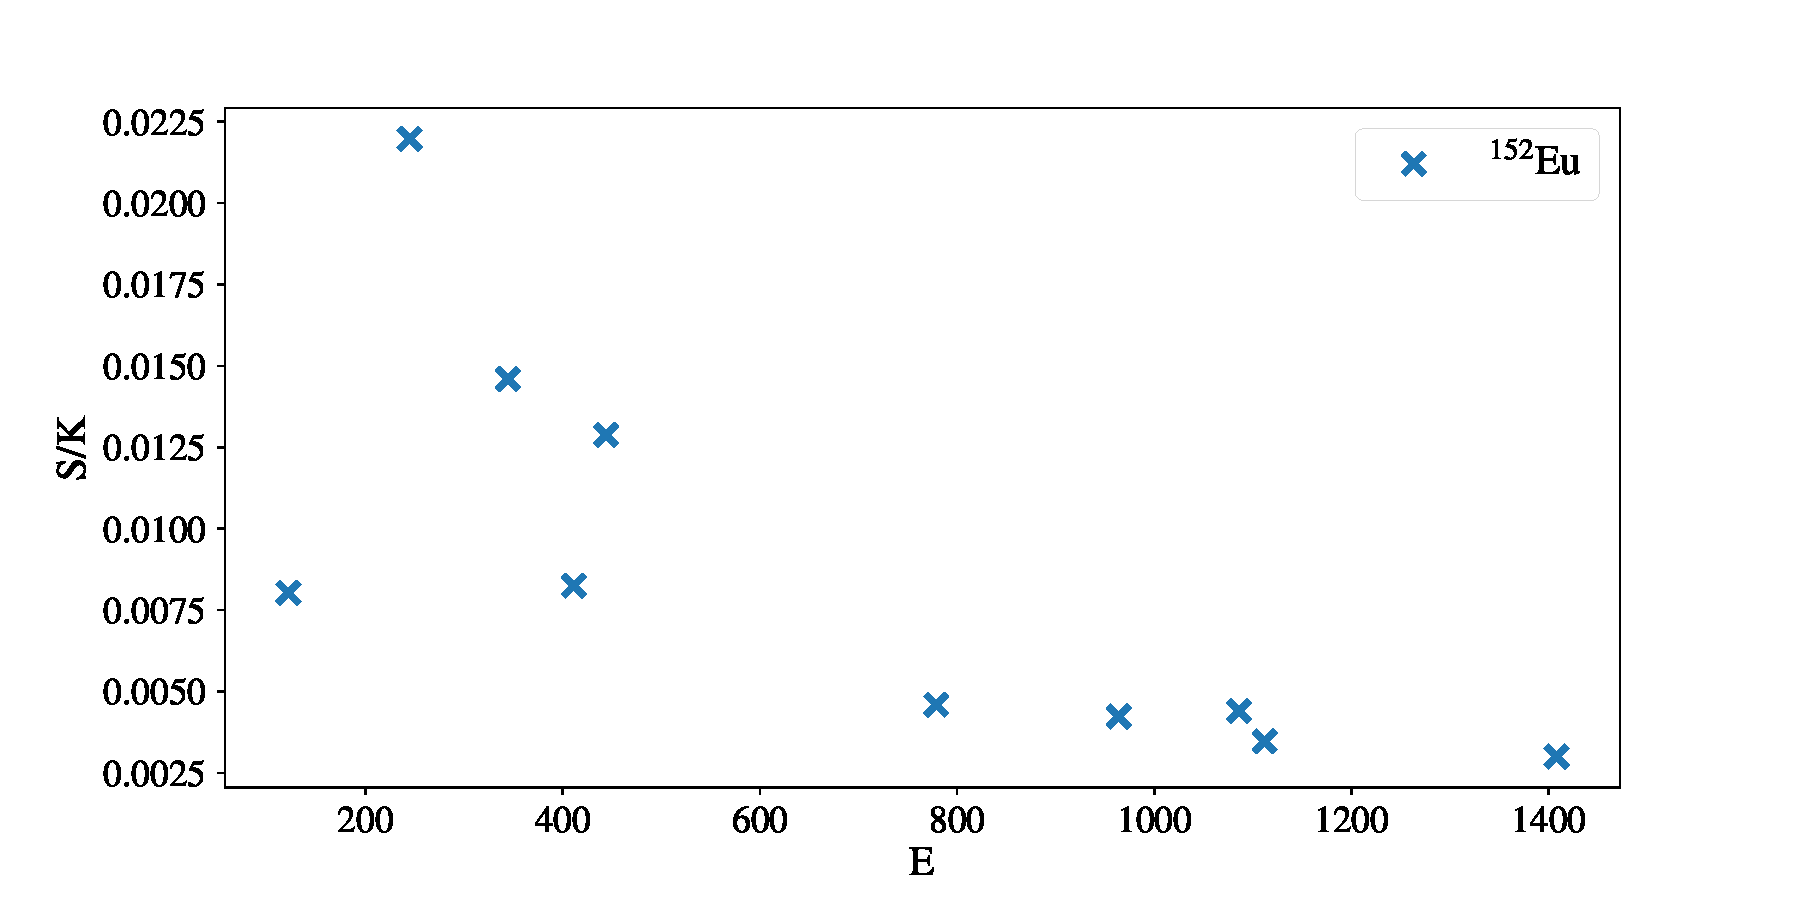
\includegraphics[width=\textwidth]{../plots/Absolute.pdf}
        \caption{$^{152}\text{Eu}$的绝对效率曲线\label{fig:Absolute}}
    \end{figure}
    \subsection{分析未知源能谱}
    在这一阶段的实验里,因为调节了放大倍数,需要重新做刻度。重新测量的$^{152}\text{Eu}$如图\ref{fig:152Eu_Half}
    \begin{figure}[htbp]
        \centering
        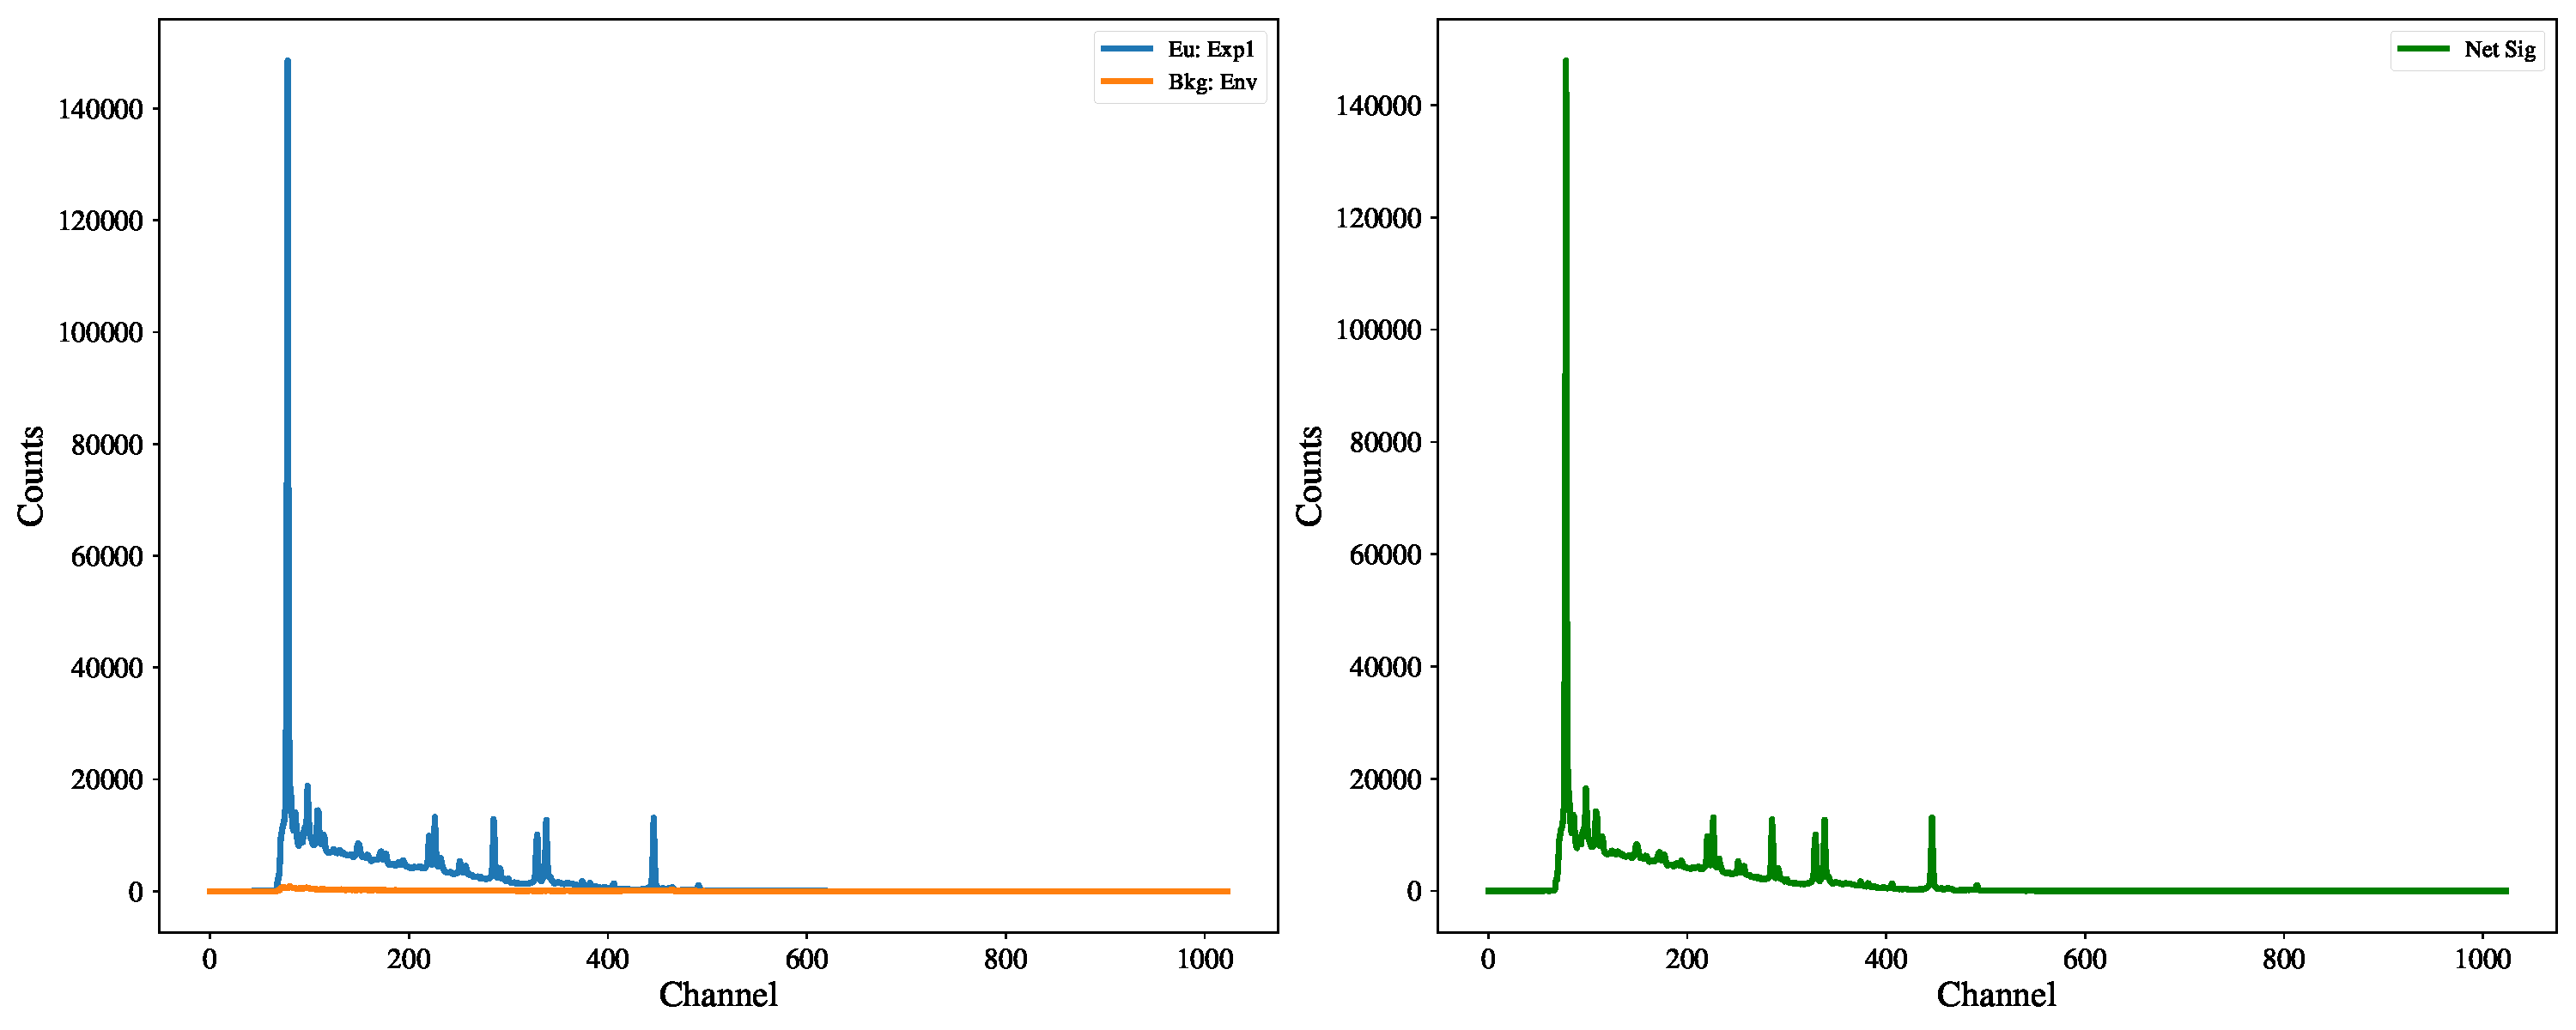
\includegraphics[width=\textwidth]{../plots/Eu_half_net.pdf}
        \caption{放大倍数缩小一半后的$^{152}\text{Eu}$测量结果\label{fig:152Eu_Half}}
    \end{figure}
    鉴于放大倍数缩小到了原来的一半,考虑到原先观察到的低能区的线性性并不好,这里我们仅考虑能量最大的四个峰进行刻度。测量结果如表\ref{tab:152Eu_half}。进行刻度,可得:\begin{equation}
        E = 2.8433*\text{Ch} + 146.2568
    \end{equation}
    线性拟合图如\ref{fig:Half_fit}。
    \begin{figure}
        \centering
        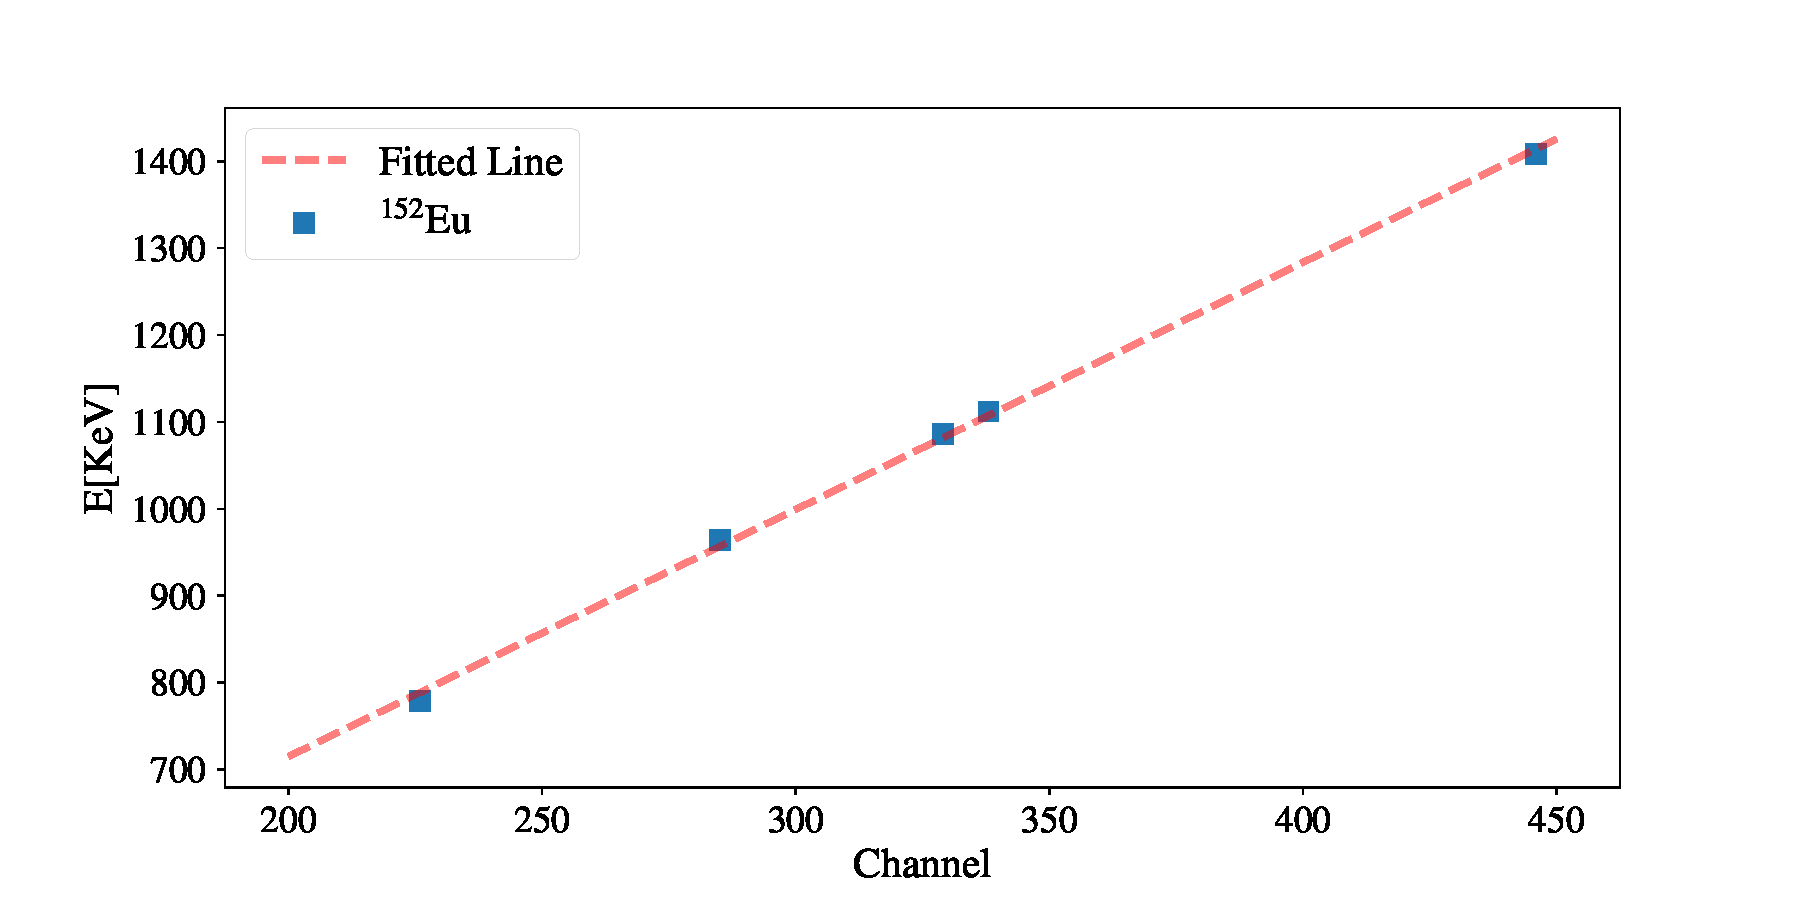
\includegraphics[width=\textwidth]{../plots/Half_fit.pdf}
        \caption{$^{152}\text{Eu}$放大倍数缩小一半后刻度结果\label{fig:Half_fit}}
    \end{figure}
    \begin{table}[htbp]
        \centering
        \caption{$^{152}\text{Eu}$放大倍数缩小一半后刻度结果\label{tab:152Eu_half}}
        \begin{tabular}{lrrrrr}
\toprule
Peak    &       1 &       2 &      3 &      4 &      5 \\
\midrule
Channel &   446 &   338 &   329&  285 &  226 \\
$E[\si{KeV}]$       &  1408.03 &  1112.0 &  1085.8 &  964.0 &  778.9 \\
\bottomrule
\end{tabular}
    \end{table}

    对环境本底和矿渣的测量图如图\ref{fig:slag_vs_env}所示。
    \begin{figure}
        \centering
        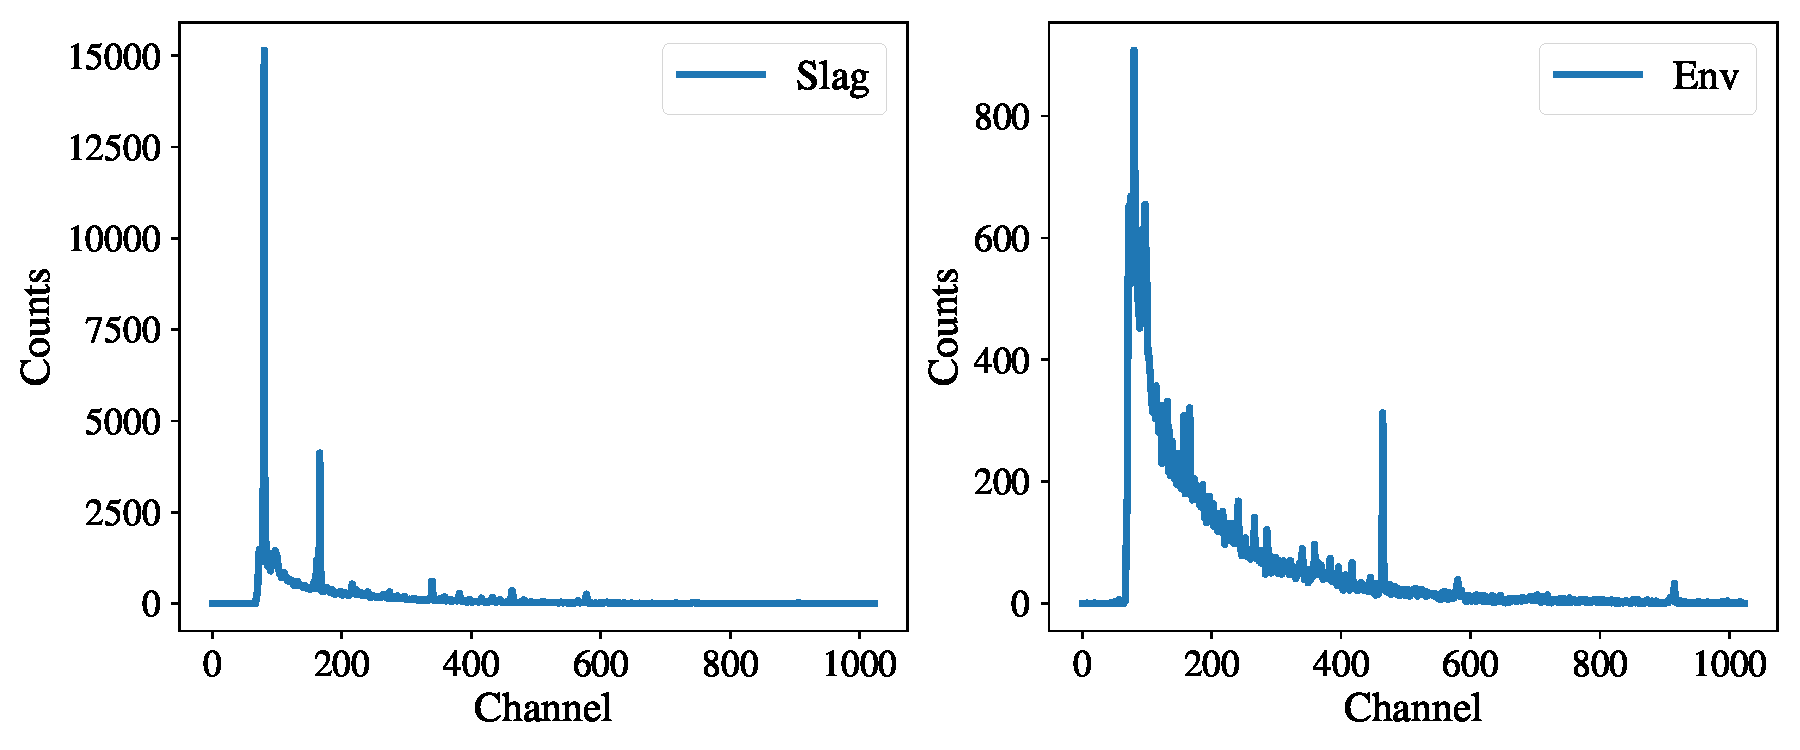
\includegraphics[width=\textwidth]{../plots/slag_vs_env.pdf}
        \caption{矿渣(左)和环境本底(右)的测量结果\label{fig:slag_vs_env}}
    \end{figure}

    对环境本底的各峰如表\ref{tab:Env_E}及图\ref{fig:Env_E}所示。
    \begin{table}[htbp]
        \centering
        \caption{环境本底测量和峰位能量表\label{tab:Env_E}}
        \begin{tabular}{lrrrrrrr}
\toprule
Peak &            1 &           2 &            3 &           4 &           5 &           6 &          7 \\
\midrule
Channel &   915.000000 &   581.00000 &   464.000000 &  286.000000 &  242.000000 &   97.000000 &   81.00000 \\
E Pred. &  2747.835006 &  1798.18789 &  1465.527074 &  959.427712 &  834.324499 &  422.052548 &  376.56047 \\
\bottomrule
\end{tabular}

    \end{table}
    \begin{figure}[htbp]
        \centering
        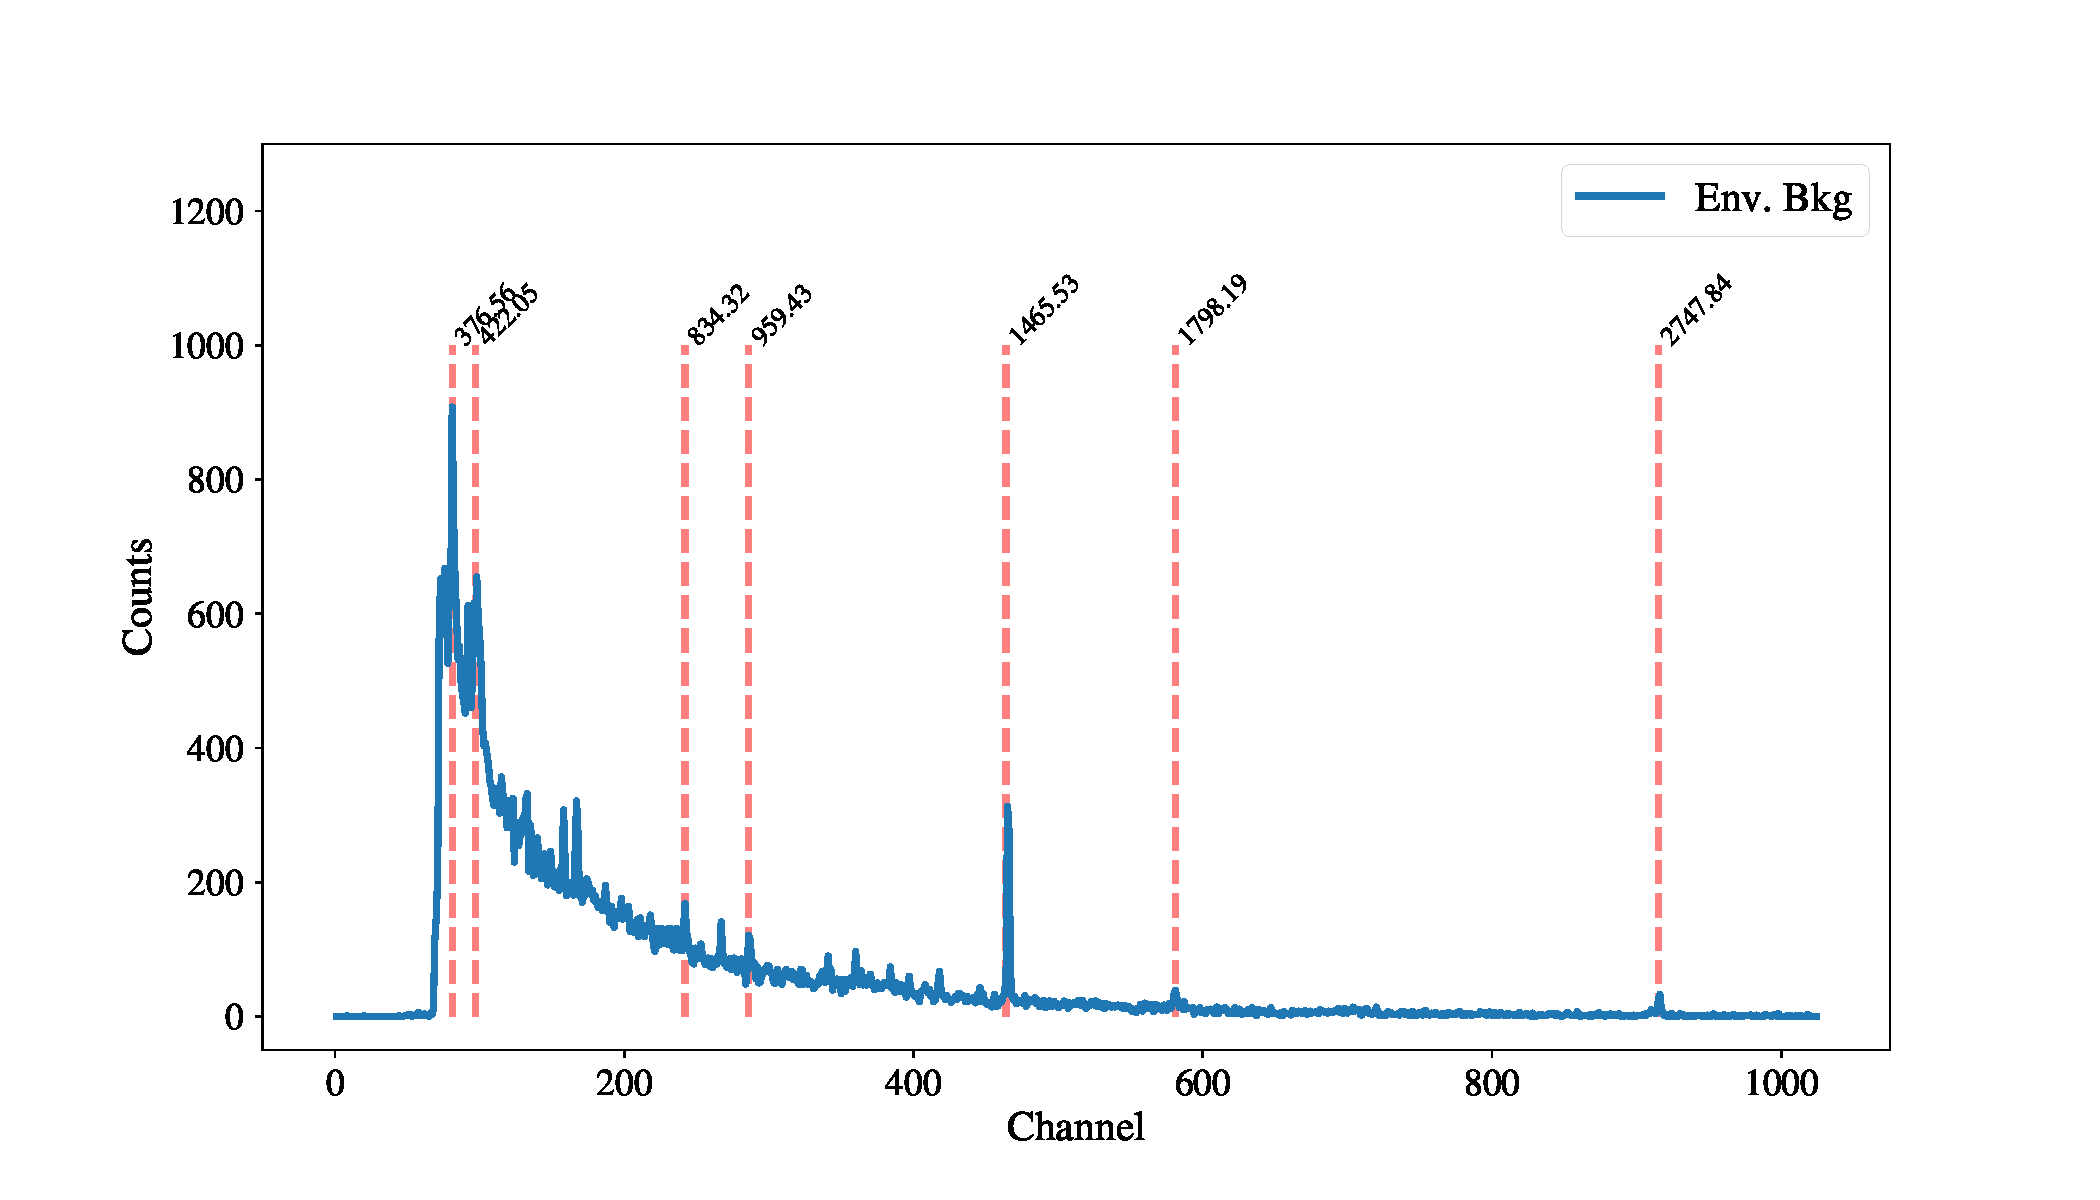
\includegraphics[width=\textwidth]{../plots/Env_E.pdf}
        \caption{环境本底测量和峰位能量图\label{fig:Env_E}}
    \end{figure}
    对矿渣样品的测量结果如图\ref{fig:Slag_E}和表\ref{tab:Slag_E}所示。
    \begin{table}[htbp]
        \centering
        \caption{矿渣信号测量和峰位能量表\label{tab:Slag_E}}
        \begin{tabular}{lrrrrrrr}
\toprule
Peak &           1 &            2 &            3 &            4 &           5 &           6 &           7 \\
\midrule
Channel &   577.00000 &   412.000000 &   380.000000 &   339.000000 &  165.000000 &   98.000000 &   80.000000 \\
E Pred. &  1786.81487 &  1317.677822 &  1226.693667 &  1110.120219 &  615.393877 &  424.895803 &  373.717216 \\
\bottomrule
\end{tabular}

    \end{table}
    \begin{figure}[htbp]
        \centering
        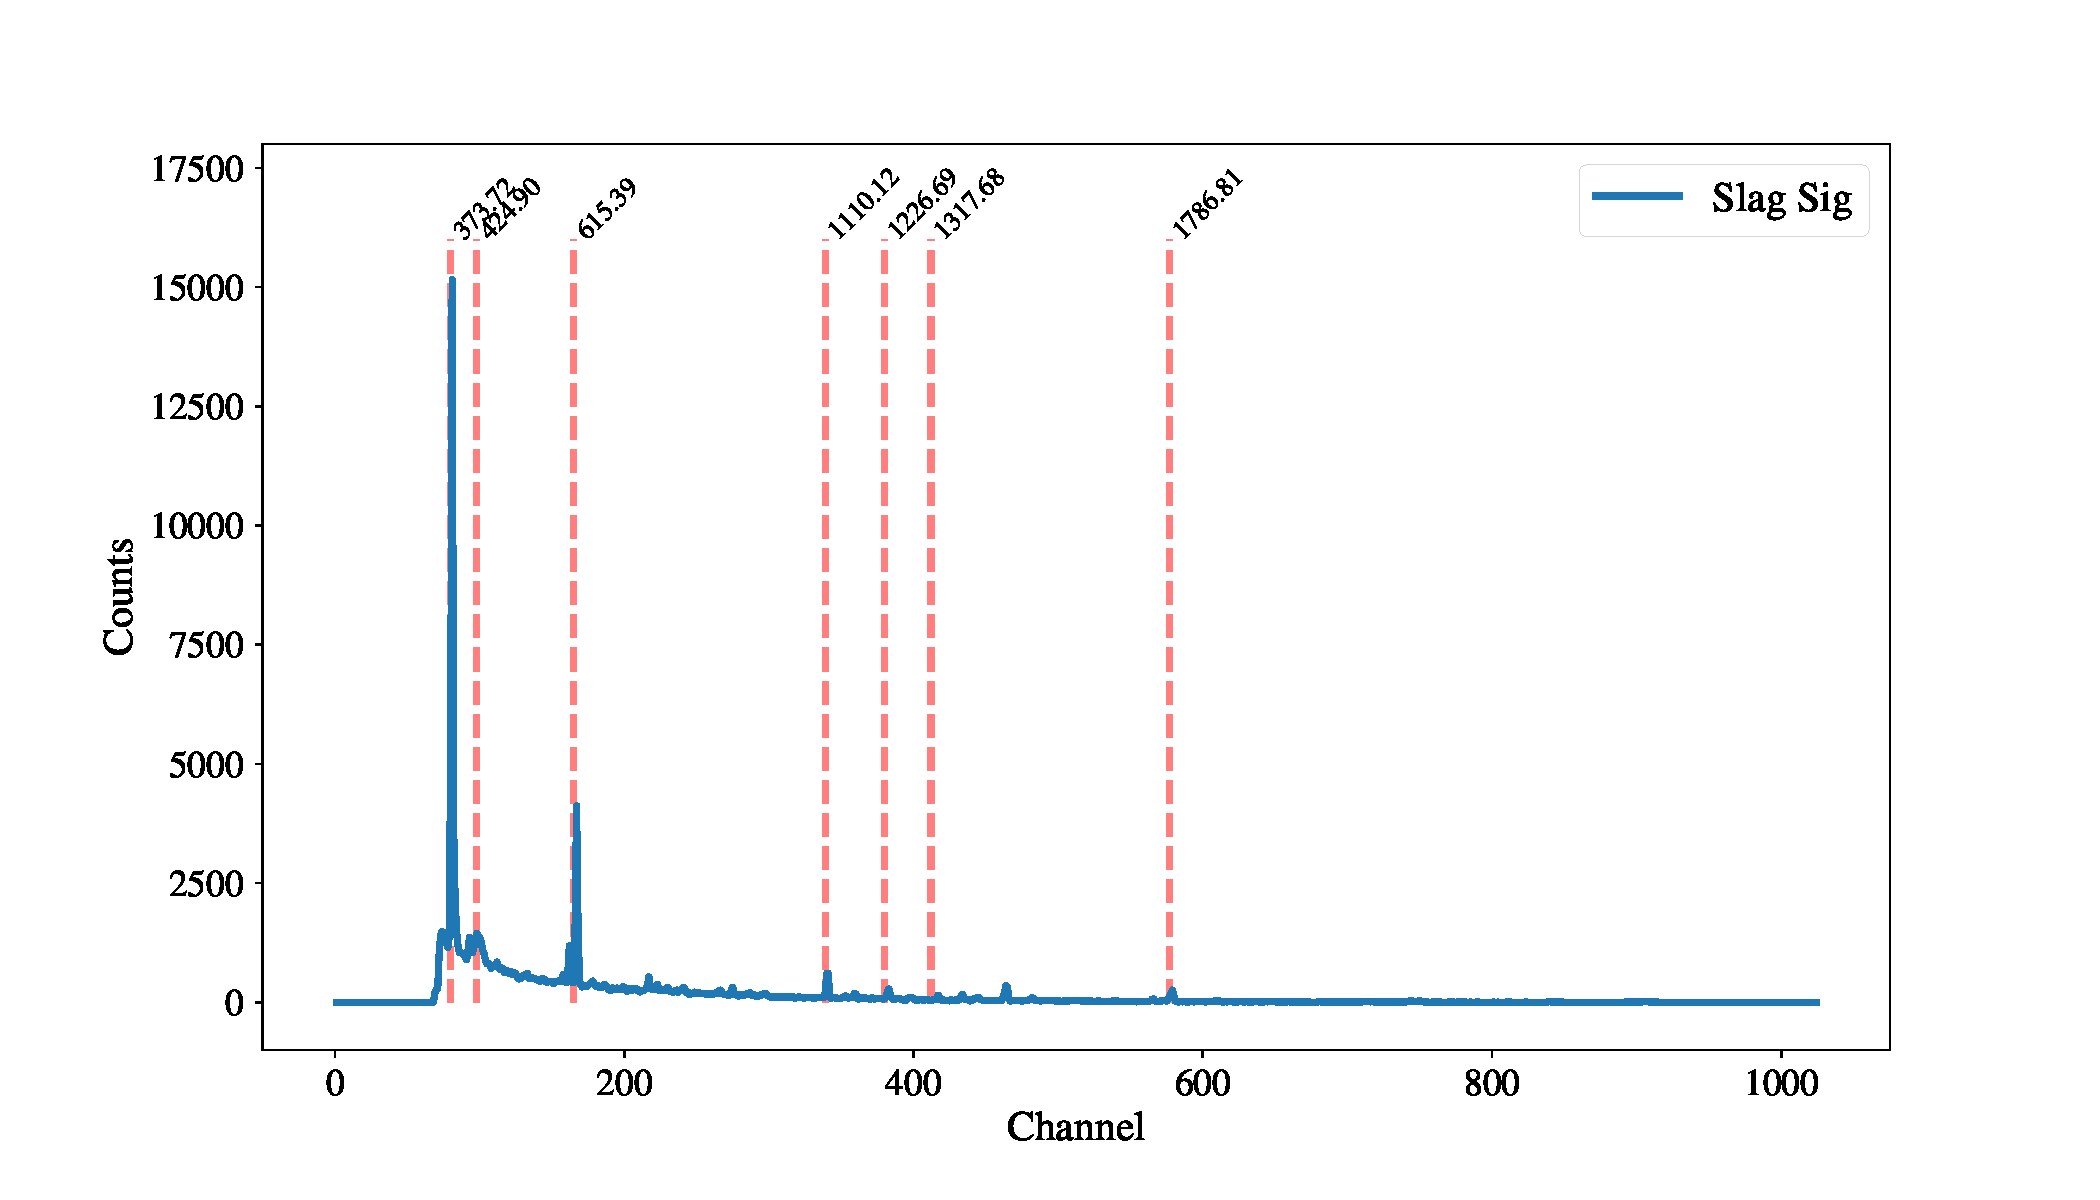
\includegraphics[width=\textwidth]{../plots/Slag_E.pdf}
        \caption{矿渣信号本底测量和峰位能量图\label{fig:Slag_E}}
    \end{figure}
    并没有在这些信号中得到一些有意义的能谱。
\section{致谢}
    感谢许金艳老师的实验指导,感谢刘寅绅同学和童星昱同学的讨论。也感谢张轩豪同学一起进行实验。
    \clearpage
    \appendix
    \appendixpage
    \section{思考题}
    \begin{enumerate}
        \item \begin{itemize}
            \item NaI(TI)探测:对$\gamma$射线,当能量大于$150\si{KeV}$时响应是线性的。其主要优点是密度大,原子序数高,对γ射线探测效率高。同时因为发光效率高,能量分辨率也较好。但必须密封使用以防止潮解。
            \item 高纯锗: 作为半导体探测器,必须用液态氮冷却条件下使用。他的优点一是空间分辨率好,分辨时间快;二是灵敏度高;三是在同样剂 量辐照下,输出的信号比电离室大。但也有能量响应差而不能做绝对测量和辐射损伤效应等缺点。
        \end{itemize}
        \item 相对效率曲线体现出不同能量下探测效率的相对大小。通过与已知活度的放射源比较可以将相对效率归一到绝对效率。
        在能量小于$2m_{e}$时,光子主要发生康普顿散射,能量会沉积在全能峰,所以探测效率随着能量增大逐渐增加。当能量大于$2m_{e}$时,开始发生电子对效应,高能量的电子和正电子可能在消耗完能量之前就从灵敏体积中逸出,在能谱中形成单逃逸峰或双逃逸峰,使全能峰的探测效率随能量增大而减小。
        \item 高纯锗探测器禁带宽度较窄($\sim 0.7\si{eV}$),需要低温真空(液氮冷却至$77\si{K}$左右)运
        行,保证锗晶体工作于半导体状态。同时,因为探测器十分灵敏,低温也可以防止电子因为温度自激发带来显著噪声。 
    \end{enumerate}
\end{document}